\documentclass[tikz,border=10pt]{article}
\usepackage[paperwidth=26cm,paperheight=8cm,margin=0.3cm]{geometry}
\usepackage{tikz}
\usetikzlibrary{arrows.meta, positioning, fit, backgrounds, calc, shapes.geometric, decorations.pathreplacing}
\pagestyle{empty}

\definecolor{srcblue}{HTML}{4A90D9}
\definecolor{vibeteal}{HTML}{2A9D8F}
\definecolor{dedupgray}{HTML}{888888}
\definecolor{gengreen}{HTML}{2EAA4F}
\definecolor{clapamber}{HTML}{E8A838}
\definecolor{embpurple}{HTML}{7B68AE}
\definecolor{mapgreen}{HTML}{1B7A3D}
\definecolor{annotgray}{HTML}{666666}

\begin{document}
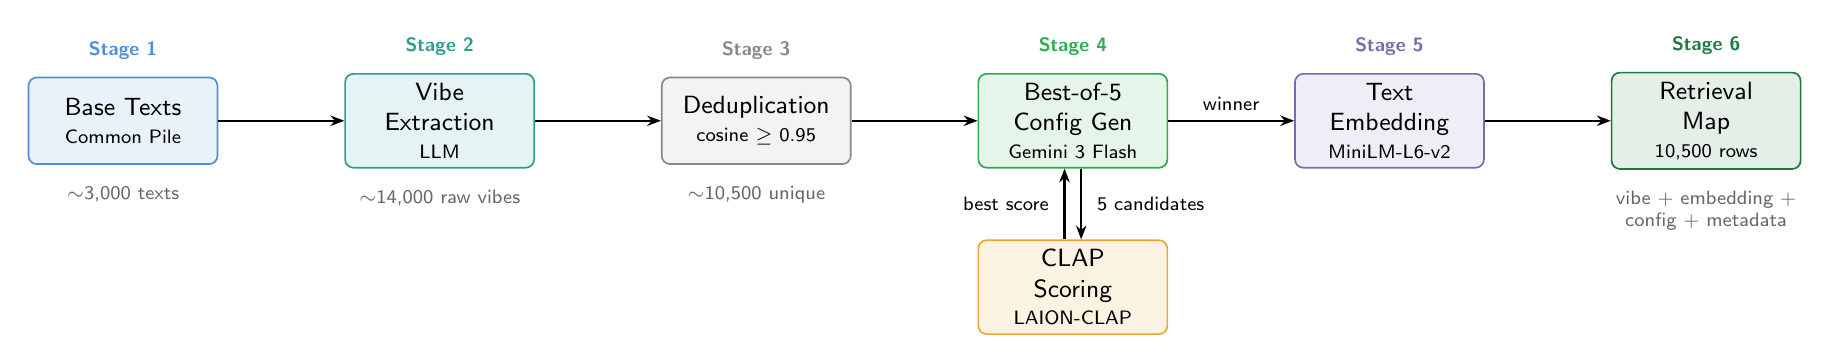
\begin{tikzpicture}[
    node distance=0.9cm and 1.2cm,
    >={Stealth[length=5pt]},
    stage/.style={draw, rounded corners=3pt, minimum height=1.1cm, minimum width=2.4cm,
                  font=\small\sffamily, align=center, line width=0.6pt},
    detail/.style={font=\scriptsize\sffamily\color{annotgray}, align=center},
    arr/.style={->, thick, line width=0.8pt},
    countlabel/.style={font=\scriptsize\sffamily\bfseries, fill=white, inner sep=1.5pt},
]

% Stage 1: Source texts
\node[stage, fill=srcblue!12, draw=srcblue] (src) {Base Texts\\[-1pt]\scriptsize Common Pile};
\node[detail, below=0.15cm of src] {$\sim$3{,}000 texts};

% Stage 2: Vibe extraction
\node[stage, fill=vibeteal!12, draw=vibeteal, right=1.6cm of src] (vibes) {Vibe\\Extraction\\[-1pt]\scriptsize LLM};
\node[detail, below=0.15cm of vibes] {$\sim$14{,}000 raw vibes};

% Stage 3: Dedup
\node[stage, fill=dedupgray!10, draw=dedupgray, right=1.6cm of vibes] (dedup) {Deduplication\\[-1pt]\scriptsize cosine $\geq$ 0.95};
\node[detail, below=0.15cm of dedup] {$\sim$10{,}500 unique};

% Stage 4: Best-of-N generation
\node[stage, fill=gengreen!12, draw=gengreen, right=1.6cm of dedup] (gen) {Best-of-5\\Config Gen\\[-1pt]\scriptsize Gemini 3 Flash};

% Stage 4b: CLAP scoring (below gen)
\node[stage, fill=clapamber!15, draw=clapamber, below=0.9cm of gen, minimum width=2.4cm] (clap) {CLAP\\Scoring\\[-1pt]\scriptsize LAION-CLAP};

% Stage 5: Embedding
\node[stage, fill=embpurple!12, draw=embpurple, right=1.6cm of gen] (embed) {Text\\Embedding\\[-1pt]\scriptsize MiniLM-L6-v2};

% Stage 6: Retrieval map
\node[stage, fill=mapgreen!12, draw=mapgreen, right=1.6cm of embed] (map) {Retrieval\\Map\\[-1pt]\scriptsize 10{,}500 rows};
\node[detail, below=0.15cm of map] {vibe + embedding +\\config + metadata};

% Arrows
\draw[arr] (src) -- (vibes);
\draw[arr] (vibes) -- (dedup);
\draw[arr] (dedup) -- (gen);

% Gen <-> CLAP loop
\draw[arr] ([xshift=3pt]gen.south) -- node[right, font=\scriptsize\sffamily, xshift=2pt] {5 candidates} ([xshift=3pt]clap.north);
\draw[arr] ([xshift=-3pt]clap.north) -- node[left, font=\scriptsize\sffamily, xshift=-2pt] {best score} ([xshift=-3pt]gen.south);

\draw[arr] (gen) -- node[above, font=\scriptsize\sffamily] {winner} (embed);
\draw[arr] (embed) -- (map);

% Stage numbers
\node[font=\scriptsize\sffamily\bfseries\color{srcblue}, above=0.1cm of src] {Stage 1};
\node[font=\scriptsize\sffamily\bfseries\color{vibeteal}, above=0.1cm of vibes] {Stage 2};
\node[font=\scriptsize\sffamily\bfseries\color{dedupgray}, above=0.1cm of dedup] {Stage 3};
\node[font=\scriptsize\sffamily\bfseries\color{gengreen}, above=0.1cm of gen] {Stage 4};
\node[font=\scriptsize\sffamily\bfseries\color{embpurple}, above=0.1cm of embed] {Stage 5};
\node[font=\scriptsize\sffamily\bfseries\color{mapgreen}, above=0.1cm of map] {Stage 6};

\end{tikzpicture}
\end{document}
